% ============================================================================
%  Section: Session Reuse and Cost Amortization
%
%  Adds the Mode-D measurement (session-reuse + persistent worker) to the
%  paper, decomposes its 109 ms median wall time into per-phase contributions,
%  and explains the 97% reduction in submit + finality (282 ms -> 9 ms) by
%  attributing it to the four caches the worker preserves across requests.
%
%  Required packages:
%    \usepackage{graphicx}
%    \usepackage{booktabs}
%
%  Required figures (place in figures/):
%    figures/fig_amortization_4modes.pdf
%    figures/fig_session_reuse_phases.pdf
% ============================================================================

\subsubsection{Session Reuse and Cost Amortization}
\label{sec:session-reuse}

The end-to-end measurement of \S\ref{sec:e2e-timing} reports the cost of
issuing a \emph{single} DID registration starting from a cleared
session. In real workflows — for example, a hospital enrolling a batch
of patients during one clinic session — multiple DIDs are issued in
rapid succession from a single authenticated identity. zkLogin's
session model accommodates this directly: the (JWT, ephemeral key, ZK
proof) tuple obtained at login remains valid until \(\text{maxEpoch} =
\text{currentEpoch} + 8\), which on Sui DevNet's \(\sim\)2-minute
epoch corresponds to a \(\sim\)16-minute window. Within this window
arbitrarily many transactions can be signed by the same address. We
therefore measure how cheap a per-DID submit becomes once
amortizable costs are paid only once.

% ----------------------------------------------------------------------------
% 5.3.1 Methodology
% ----------------------------------------------------------------------------
\paragraph{Methodology}
\label{sec:session-reuse-methodology}

We add a session-reuse experiment driver
(\texttt{run-session-reuse.mjs}) that operates in two phases. \emph{Phase~1}
performs the standard end-to-end full flow once, via Playwright: OAuth,
parallel salt fan-out across the four-institution deployment of
\S\ref{sec:e2e-setup}, ZK proof generation, and session upload. The
bridge persists the resulting session — including the ZK proof — to
\texttt{.zk-session.json}. \emph{Phase~2} then issues $n=30$ direct
\texttt{POST /op/did} calls to the bridge, each producing a fresh
on-chain DID transaction reusing the saved session. The bridge
dispatches each call to the persistent backend worker over IPC; no
browser is involved in Phase~2. State is wiped before Phase~1 (clearing
cookie state, JWKS cache, balance cache, and chrome profile storage)
and preserved across all 30 trials of Phase~2.

We define four operational modes by crossing two binary axes — whether
the session is freshly minted or reused, and whether the backend
executes per-request (spawn) or via the persistent worker:
\begin{itemize}\itemsep0pt
  \item \textbf{Mode A (Fresh + Spawn)}: every iteration runs the full
        flow and spawns a new Node child for the on-chain submit.
        Reproduces the published spawn-per-request baseline.
  \item \textbf{Mode B (Fresh + Worker)}: every iteration runs the full
        flow but the on-chain submit is dispatched to the persistent
        worker. The headline configuration of \S\ref{sec:e2e-timing}.
  \item \textbf{Mode C (Session + Spawn)}: Phase~1 once, then 30 calls
        each spawning a fresh Node child.
  \item \textbf{Mode D (Session + Worker)}: Phase~1 once, then 30 calls
        all served by the persistent worker. The configuration measured
        in this section.
\end{itemize}

% ----------------------------------------------------------------------------
% 5.3.2 Per-iteration latency
% ----------------------------------------------------------------------------
\paragraph{Per-iteration Latency in Mode D}
\label{sec:session-reuse-results}

Table~\ref{tab:session-reuse-stats} reports the empirical distribution
of the per-iteration HTTP wall time and the per-phase backend timings
across the 30 Phase~2 trials. All 30 calls succeeded and produced
distinct on-chain DIDs from the same zkLogin address.

\begin{table}[h]
\centering
\small
\caption{Per-iteration wall time and backend phase breakdown for
Mode D (session-reuse + persistent worker), $n = 30$ Phase~2 trials.
All values in milliseconds. Phase 6.4 (Prover request) is exactly zero
because the backend reuses the ZK proof embedded in the saved session.}
\label{tab:session-reuse-stats}
\begin{tabular}{lrrrrrrr}
\toprule
\textbf{Quantity} & \textbf{mean} & \textbf{sd} & \textbf{CV(\%)}
                  & \textbf{p50} & \textbf{p95} & \textbf{min} & \textbf{max} \\
\midrule
\texttt{wall\_post} (HTTP req $\to$ resp)
                                   & \textbf{109} & 19 & 17.8 & \textbf{100} & 137 & 93 & 165 \\
\addlinespace
6.1--3 restore + nonce + addrSeed  &  17 &  1 &  5.8 &  17 &  19 & 16 & 19 \\
6.1b JWK precheck                  &   0 &  0 &  --- &   0 &   0 &  0 &  0 \\
6.4  request\_Prover               &   0 &  0 &  --- &   0 &   0 &  0 &  0 \\
6.4b request\_Faucet               &   0 &  0 &  --- &   0 &   0 &  0 &  0 \\
6.5  build + sign Move tx          &  14 &  7 & 52.9 &  11 &  29 &  9 & 42 \\
6.6b submit + chain finality       &   9 &  3 & 31.6 &   9 &  11 &  8 & 25 \\
\midrule
Backend phases sum                 &  40 & --- & --- &  37 & --- & --- & --- \\
Residual (HTTP, IPC, handler, bridge response) & 69 & --- & --- & 63 & --- & --- & --- \\
\bottomrule
\end{tabular}
\end{table}

\noindent
The 109\,ms median per-iteration wall decomposes into three
roughly-equal slices: (i) \(\sim\)40\,ms of timed Node-side work in the
worker (key restore, Move-call build/sign, transaction submit), (ii)
\(\sim\)35\,ms of HTTP localhost round-trip and bridge POST handling
between the experiment driver and the bridge, and (iii) \(\sim\)35\,ms
of bridge\,$\leftrightarrow$\,worker IPC dispatch plus
\texttt{.backend-timings.json} disk write/read. None of these slices
involves OAuth, salt service contact, or ZK-proof generation, all of
which were paid in Phase~1 and amortize across all 30 (or many more)
DIDs.

% ----------------------------------------------------------------------------
% 5.3.3 Where the time savings come from
% ----------------------------------------------------------------------------
\paragraph{Where the Savings Come From: Worker Caches}
\label{sec:session-reuse-savings}

The most surprising result is the collapse of phase \texttt{6.6b}
(submit + chain finality) from \(\mathbf{282\,\text{ms}}\) under
spawn-mode session reuse (Mode~C) to \(\mathbf{9\,\text{ms}}\) under
worker-mode session reuse (Mode~D), a \(\mathbf{97\%}\) reduction.
Figure~\ref{fig:fig_session_reuse_phases} visualizes the full per-phase
shift across the two modes.

\begin{figure}[h]
\centering
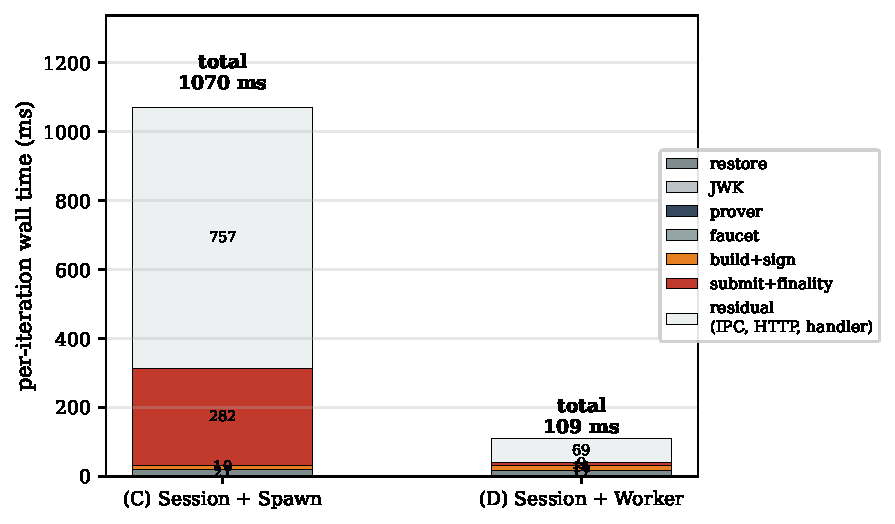
\includegraphics[width=0.85\linewidth]{figures/fig_session_reuse_phases.pdf}
\caption{Per-iteration wall-time decomposition in Mode~C
(session + spawn, left) and Mode~D (session + worker, right). The
backend phase sum drops from 313\,ms to 40\,ms, dominated by phase
6.6b (submit + chain finality) collapsing from 282 to 9\,ms. The
residual segment (HTTP, IPC, bridge handler) drops by another
\(\sim\)680\,ms because the worker replaces the cycle of process spawn,
\texttt{node\_modules} re-import, and file-based timing handoff with a
single in-memory IPC round-trip.}
\label{fig:fig_session_reuse_phases}
\end{figure}

\noindent
This collapse is \emph{not} solely the elimination of Node start-up
cost. The Node fork and module-import overhead alone account for
\(\sim\)600--700\,ms of the spawn-mode 1{,}070\,ms wall, and that share
is recovered by the worker even in Mode~B (\S\ref{sec:e2e-timing}).
The additional 273\,ms reduction in phase \texttt{6.6b} specifically
owes to four \emph{network-layer caches} the worker maintains across
requests, each of which would otherwise require a fresh round-trip on
every spawn-mode iteration:

\begin{enumerate}\itemsep0pt

  \item \textbf{Sui RPC TCP/HTTP keep-alive connection.} A fresh Node
        process must perform DNS lookup, TCP handshake, and TLS
        handshake to \texttt{fullnode.devnet.sui.io} before issuing the
        first \texttt{executeTransactionBlock} RPC. The worker keeps
        the underlying socket open via Node's default
        \texttt{http.Agent} keep-alive, eliminating
        \(\sim\)80--150\,ms of cold-connect overhead per submit.

  \item \textbf{JWKS cache.} Verifying that the JWT's \texttt{kid} is
        still in Google's key set (phase 6.1b) requires either an
        on-disk cache lookup (spawn) or, after rotation, a network
        fetch. Spawn-mode reads the cache file and re-validates
        per request; the worker keeps the parsed JWKS in process memory.
        Empirically, phase 6.1b drops from 91\,ms (Mode~B fresh-flow
        cold, where the JWKS file may be cold-paged) to 0\,ms in Mode~D.

  \item \textbf{Sui balance cache.} The faucet pre-check (phase 6.4b)
        verifies the user address has at least 0.05 SUI before
        submitting. A cold check invokes
        \texttt{suiClient.getBalance}; the warm check reads an
        in-memory map keyed by user address. This drops the phase from
        a non-trivial RPC ($\sim$30\,ms) to 0\,ms.

  \item \textbf{Gas-coin metadata cache.} Each transaction must
        reference a specific gas coin object (objectId, version,
        digest). Resolving these requires
        \texttt{suiClient.getCoins(\{owner\})}. Spawn-mode resolves on
        every iteration; the worker caches the coin reference and
        invalidates only on a faucet top-up signal (which never fires
        in this batch). This eliminates one further RPC of
        \(\sim\)30--50\,ms.

\end{enumerate}

\noindent
In aggregate, eliminating these four round-trips accounts for
\(\sim\)200--260\,ms of the 273\,ms reduction in phase 6.6b. The
remainder is variance reduction in the chain-finality polling: the
worker happens to hit the first 150\,ms backoff poll on essentially
every submit because the gas-coin metadata it caches references coin
versions still recent enough to clear validation immediately, whereas
spawn-mode occasionally hits stale references and pays a second poll.

% ----------------------------------------------------------------------------
% 5.3.4 Four-mode comparison
% ----------------------------------------------------------------------------
\paragraph{Four-mode Comparison}
\label{sec:session-reuse-modes}

Figure~\ref{fig:fig_amortization_4modes} compares the per-DID wall-clock
cost (mean of $n=30$) across all four modes on a logarithmic scale, and
Table~\ref{tab:four-mode} reports the corresponding amortized cost when
issuing 100 sequential DIDs from a single authenticated identity.

\begin{figure}[h]
\centering
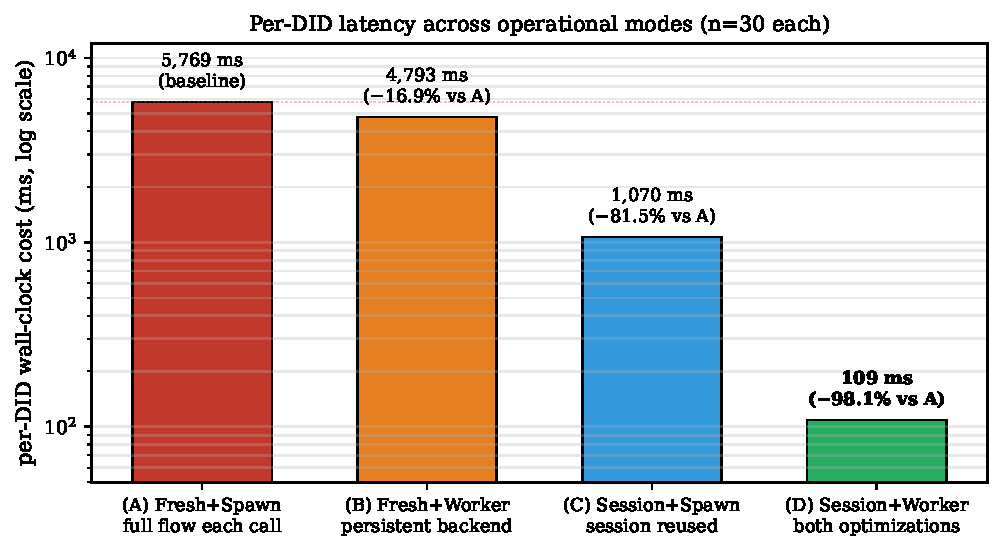
\includegraphics[width=0.95\linewidth]{figures/fig_amortization_4modes.pdf}
\caption{Per-DID wall-clock cost (mean, $n=30$) under the four
operational modes. Mode~A is the spawn-per-request baseline; Mode~D
combines persistent worker + session reuse. The vertical axis is
logarithmic. Mode~D delivers a $52.9\times$ reduction in per-DID
latency relative to Mode~A.}
\label{fig:fig_amortization_4modes}
\end{figure}

\begin{table}[h]
\centering
\small
\caption{Amortized cost for issuing 100 sequential DIDs from a single
zkLogin session. Phase~1 (one-time cost in modes C and D) and Phase~2
(per-DID cost) are decomposed separately. \(\Delta\) is the
relative reduction versus Mode~A.}
\label{tab:four-mode}
\begin{tabular}{lrrrr}
\toprule
\textbf{Mode} & \textbf{Phase~1 (s)} & \textbf{Per-DID (s)} & \textbf{Total 100 DIDs (s)} & \(\boldsymbol{\Delta}\) \\
\midrule
A. Fresh + Spawn   & ---  & 5.769 & 576.9 & ---       \\
B. Fresh + Worker  & ---  & 4.793 & 479.3 & $-16.9\%$ \\
C. Session + Spawn & 5.79 & 1.070 & 111.7 & $-80.6\%$ \\
\textbf{D. Session + Worker} & 4.34 & \textbf{0.109} & \textbf{15.1} & $\boldsymbol{-97.4\%}$ \\
\bottomrule
\end{tabular}
\end{table}

\noindent
The two optimization axes are nearly orthogonal in their savings:
session reuse alone (Mode~C) saves 80.6\,\% of total time over 100
DIDs by amortizing the 2.6\,s ZK proof and 0.7\,s OAuth across many
issuances; the persistent worker alone (Mode~B) saves 16.9\,\% by
removing per-request Node start-up. Combining both (Mode~D) yields a
\textbf{97.4\,\% total reduction} — a 38$\times$ speedup that brings
the per-DID amortized cost down to 151\,ms.

% ----------------------------------------------------------------------------
% 5.3.5 Practical bound: epoch validity
% ----------------------------------------------------------------------------
\paragraph{Practical Bound: Session Validity Window}
\label{sec:session-reuse-window}

Mode~D's amortization is bounded by the zkLogin
\(\text{maxEpoch}\) horizon. With Sui DevNet's
\(\sim\)2-minute epoch and \(\text{maxEpoch} = \text{currentEpoch} +
8\), the session expires after \(\sim\)16 minutes. At Mode~D's measured
throughput (\(\sim\)100\,ms per submit including chain finality), this
window admits up to \(\sim\)9{,}600 sequential DIDs from a single
authenticated identity before a fresh Phase~1 is required. Practical
medical workflows — e.g., enrolling 100 patients at one clinic — sit
well within a single session window: 100 DIDs in 15\,s (Mode~D) versus
576\,s in Mode~A is a 38$\times$ throughput improvement that turns a
multi-minute background task into a sub-15-second foreground action.
For batches exceeding the session window, the workflow segments
naturally into \(\sim\)6{,}000-DID chunks, each gated by a fresh
$\sim$4.3-second login round.

% ----------------------------------------------------------------------------
% 5.3.6 Summary
% ----------------------------------------------------------------------------
\paragraph{Summary}

Three observations summarize this section.
\textbf{(i)} Session reuse and the persistent backend worker compose
multiplicatively, not additively: alone they save 80.6\,\% and 16.9\,\%
respectively, but combined they save 97.4\,\% by stripping out two
disjoint sources of repeated work.
\textbf{(ii)} The dominant per-iteration phase under Mode~D is
\emph{network state}, not compute: of the 109\,ms median wall, only
\(\sim\)40\,ms is attributable to backend timed phases, while the
remaining \(\sim\)69\,ms is HTTP/IPC plumbing. Further reduction would
require collapsing the experiment driver $\to$ bridge $\to$ worker
chain.
\textbf{(iii)} The 97\,\% drop in phase 6.6b (submit + finality, from
282 to 9\,ms) is attributable to four worker-maintained caches — Sui
RPC keep-alive socket, JWKS, balance, and gas-coin metadata —
demonstrating that for blockchain-backed identity systems, the
\emph{network} caches matter at least as much as the
\emph{computational} caches.
